% !TeX root = ../main.tex

\chapter{Data Structures}
Data structures


We can class Data structures into two distinct category's based on whether or not they use pointers:
\begin{itemize}
	\item \textit{Contiguously-allocated structures} are composed of single slabs of memory, and include arrays, matrices, heaps and hash tables
	\item \textit{Linked data structures} are composed of distinct chunks of memory bound together by \textit{pointers} and include lists, trees and graph adjacency lists.
\end{itemize}

\section{Arrays}
	The \textit{array} is the fundamental contiguously-allocated data structure. Arrays are structures of fixed-size data records such that each element can be efficiently located by its \textit{index}.

	There are several advantages to using contiguously-allocated arrays:
	\begin{description}
		\item[Constant-time access given the index] - Because the index of each element maps directly to a particular memory address, we can access arbitray data tiems instantly provided we know the index.
		\item[Space Effciency] - Arrays consist purely of data, sono space is wasted with links or other formatting information. Further, end-of-record information is not needed because arrays are built from fixed-size records
		\item[Memory locality] - A common programming idiom involves iterating through all the elements of a data structure. Arrays are good for this because they exhibit excellent memory locality. Physical continuity between successive \textit{cache memory} in modern computer architectures
	\end{description}

	The disadvantages of arrays is that we cannot adjust their size in the middle of a programs' execution. Our program will fail soon as we try to add the $(n+1)$ customer, if we have only allocated room for $n$ records. We could compensate by allocating extremely large arrays, but this can waste space, restricting what our programs actually do.

	\subsection{Dynamic Arrays}
		Dynamic Arrays are a way around the restriction placed by arrays being fixed size. With a dynamic array we enlarge arrays as we need them. Suppose we start with an array of size 1, and double its size from $m$ to $2m$ each time we run out of space. This doubling process involves allocating a new array of size $2m$, copying the contents of the old array to the lower half of the new one, and returning the space used by the old array to the storage allocation system. Snippet. \ref{code:doubleArray} shows an implementation that takes an array and a size and returns a new array.
\begin{listing}[h]
	\begin{minted}{c}
int* double_array(int *array, int size) {
	int i;
	int* new_array = malloc(sizeof(int) * 2 * size);
	for(i = 0; i < size; i++) {
		new_array[i] = array[i]
	}
	free(array);
	return new_array;
}
	\end{minted}
	\caption{\label{code:doubleArray} Implementing a dynamic array in C}
\end{listing}

	On average each of the $n$ elements in the array only move $2n$ times, so the total work is the on the order of \bigO{n}. Adding a new element to an array no longer takes constant time \textit{in the worst case} instead all querys will be fast, except for those relatively few queries triggering array doubling.

\section{Linked Lists}
	Linked lists are one of the fundemental data structures which are often extended to make complex structures.
\begin{listing}[h]
	\begin{minted}{c}
typedef struct list {
	item_type  item; // data item
 	struct list *next; // pointer to successor
}
\end{minted}
	\caption{\label{code:linkedlist} Linked List declaration}
\end{listing}
	All linked data structures share certain properties as shown in snippet \ref{code:linkedlist}. In particular:
	\begin{itemize}
		\item Each node in our data structure (here \texttt{list}) contains one or more data fields (here \texttt{item}) that retain the data that we need to store
		\item Each node contains a pointer field to at least one other node (here \texttt{next}). This means that much of the space used in linked data structures has to be devoted to pointers, not data.
		\item Finally, we need a pointer to the head of the structure so that we know where to start.
	\end{itemize}

	The list is the simplest linked structure. The three basic operations supported by lists are searching, insertion and deletion. In doubly-linked lists, each node points to both its successor and its predecessor

	\begin{figure}[h]
		\centering
		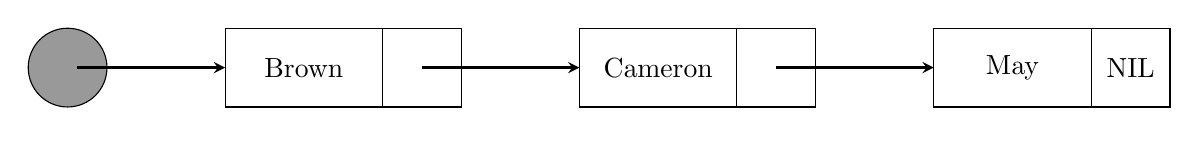
\begin{tikzpicture}
		\draw [fill=gray!80]  (-5,0.5) node (v4) {}  ellipse (0.5 and 0.5);
		\draw  (-3,1) rectangle (-1,0) node (v1) {};
		\draw  (v1) rectangle (0,1);
		\draw  (1.5,1) rectangle (3.5,0) node (v2) {};
		\draw  (v2) rectangle (4.5,1);
		\draw  (6,1) rectangle (8,0) node (v3) {};
		\draw  (v3) rectangle (9,1);
		\draw[-stealth, thick] (-0.5,0.5) -> (1.5,0.5);
		\draw[-stealth, thick]  (4,0.5) -- (6,0.5);
		\draw[-stealth, thick]  (v4) -- (-3,0.5);
		\node at (-2,0.5) {Brown};
		\node at (2.5,0.5) {Cameron};
		\node at (7,0.5) {May};
		\node at (8.5,0.5) {NIL};
		\end{tikzpicture}
		\caption{\label{fig:singlylinkedlist} a singly linked list for the 3 most recent prime minsters}
	\end{figure}

	\subsection{Searching a List}
		Searching for item $x$ in a linked list can be done either utilising iteration or recursion. Snippet. \ref{code:search_list} is an example of a recursive implementation. If $x$ is in the list it is either in the first item or it is located in the smaller rest of the list. Eventually we will reach a point where we have an empty list. Clearly $x$ cannot be there so we can return $NULL$.
	\begin{listing}[h!]
		\begin{minted}{c}
list* search_list(list *l, item_type x) {
	if (l == NULL) {
		return(NULL);
	}

	if (l->item == x) {
		return(l);
	} else {
		return( search_list(l->next, x));
	}
}
\end{minted}
	\caption{\label{code:search_list} Searching for item $x$ in list $l$}
\end{listing}

		\subsection{Insertion into a list}
			Insertion into a list is. We have no particular need at this moment to maintain the list in any particular order so we can instead choose to insert each new item where ever is easiest. In a singly linked list this is the beginning as it avoids any need to traverse the list, but does require us to update the pointer at the end of the list, denoted $l$. Snippet. \ref{code:insert_list} shows the pointer manipulation required. Just a quick note, the double star ($\texttt{**l}$) denotes that $l$ is a \textit{pointer to a pointer} to a list node. Thus the last line, \texttt{*l=p;}, copies $p$ to the place pointed to by $l$, which is the external variable maintaining access to the head of the list.

\begin{listing}[h!]
	\begin{minted}{c}
void insert_list(list **l, item_type x) {
	list *p; /* temporary pointer */
	p = malloc( sizeof(list));
	p-> item = x;
	p-> next = *l;
	*l = p;
}
\end{minted}
	\caption{\label{code:insert_list} Inserting item $x$ into list $l$}
\end{listing}

	\subsection{Deletion from a List}
		Deletion from a linked list is a bit more complicated than insertion. First we don't have the luxury of just deleting where ever is easiest. Instead we have to search to find the pointer to the \textit{predeccessor} of the item to be deleted. Snippet. \ref{code:predecessor_list} shows how we can use recursion to find the necessary pointer.

\begin{listing}[h!]
	\begin{minted}{c}
list predecessor_list(list *l, item_type x) {
	if((l == NULL) || (l->next == NULL)) {
		retur(NULL);
	}

	if ((l->next)->item == x) {
		return(l);
	} else {
		return( predecessor_list(l->next, x));
	}
}
\end{minted}
	\caption{\label{code:predecessor_list} Finding the predecessor to item $x$ in list $l$}
\end{listing}

Now that we have found the pointer to the doomed node, the actual deletion operation is simple, once ruling out the case that the to-be-deleted element doesn't exist. Note that special care should be taken to reset the pointer to the head of the list ($l$) when the first element is deleted.

\begin{listing}[h!]
	\begin{minted}{c}
void delete_list(list **l, item_type x) {
	list *p;			/* item pointer */
	list *pred; 		/* predecessor pointer */
	list *search_list(), *predecessor_list();

	p= search_list(*l, x);
	if (p != NULL) {
		pred = predecessor_list(*l, x);
		if (pred == NULL) {
			*l = p->next; /* Case when x is head */
		} else {
			pred->next = p->next;
		}
		free(p);
	}
}
\end{minted}
	\caption{\label{code:delete_list} Deleting item $x$ from list $l$}
\end{listing}

\section{Comparison of Arrays and Linked Lists}
	The relative advantages of linked lists over static arrays include:
		\begin{itemize}
			\item Overflow on linked structures can never occur unless memory is actually full.
			\item Insertions and deletions are simpler than for contiguous (array) lists.
			\item With large records, moving pointers is easier and faster than moving the items themselves
		\end{itemize}
	The relative advantages of arrays include:
	\begin{itemize}
		\item Linked structures require extra space for storing pointer fields.
		\item Linked lists do not allow efficient random access to items
		\item Arrays allow better memory locality and cache performance than random pointer jumping.
	\end{itemize}

\section{Fields, Records and Files}
	
	\subsection{Fields and Records}
	
	\subsection{Text Files}
		\subsubsection{CSV}
		
		\subsubsection{XML}
		
		\subsubsection{JSON}
		
	\section{Binary Files}
\section{Abstract Data Types}
\section{Stacks and Queues}
	Stacks and Queues are often called \textit{containers}, denoting that they are data structure that permits storage and retrieval of data items \textit{independent of content}. We distinguish between containers by the particular retrieval order that they support.
	\begin{description}
		\item[Stacks] Support retrieval by last-in, first-out (LIFO) order. Stacks are simple to implement and very efficient For this reason stacks are probably the best container to use when retrieval order doesn't matter. The \textit{put} and \textit{get} operations are often called \textit{push} and \textit{pop}.
		\item[Queues] Support retrieval by first in, first out (FIFO) order. This is usually the fairest way to control waiting times for services. You want the container holding jobs ina FIFO order to minimize the \textit{maximum} time spent waiting. Queues are somewhat trickier to implement than stacks and thus are more appropriate for applications where the order is important. The \textit{put} and \textit{get} operations are often called \textit{enqueue} and \textit{dequeue}.
	\end{description}

	Stacks and queues can be effectively implemented using either arrays or linked lists. The key issue is whether an upper bound on the size of the container is known in advance.

\section{Dictionaries}
	The \textit{dictionary} data type permits access to data items by content. You stick an item into a dictionary so you can find it where you need it. The primary operations of dictionary support are:
	\begin{itemize}
		\item \textit{Search(D,k)} - Given a search key, $k$, return a pointer to the element in dictionary $D$ whose key value is $k$, if one exists.
		\item \textit{Insert(D,x)} - Given a data item $x$, add it to the set in the dictionary $D$.
		\item \textit{Delete(D,k)} - Given a pointer to a given data item $x$ in the dictionary $D$, remove it from $D$.
	\end{itemize}

	Certain dictionary data structues also efficently support other useful operations:
		\begin{itemize}
			\item \textit{Max(D) or Min(D)} - Retrieve the item with the largest (or smallest) key from $D$. This enables the dictionary to serve as a priority queue.
			\item \textit{Predecessor(D,x) or Successor(D,x)} - Retrieve the item from D whose key is immediately before (or after) $x$ in sorted order. This allows us to iterate through the elements of the data structure.
		\end{itemize}
	\subsection{Using a List or an Array?}

		In this section we will look at the advantages and disadvantages or using arrays or linked list for implementing a Dictionary. There are more complicated approaches using binary search trees and hash tables which we will come across shortly. Table \ref{tab:BigODictionary} shows a comparison of the worst case performance of the basic dictionary operations. We will discuss the results of this and the implementations of each of the operations to fully grasp it.
		\begin{table}[h]
				\centering
				\renewcommand{\arraystretch}{1.5}
			\begin{tabular}{M{0.25\linewidth} | M{0.12\linewidth} |M{0.12\linewidth} |M{0.12\linewidth} |M{0.12\linewidth} |M{0.12\linewidth}|M{0.12\linewidth}}
				Dictionary Operations & Unsorted Array & Sorted Array & Singly Unsorted List & Doubly Unsorted List & Singly Sorted List & Double Sorted List \\
				\hline \hline
	$Search(L, k)$ 		& \bigO{n} 	& \bigO{\log n}	& \bigO{n}	& \bigO{n} 	& \bigO{n} 	& \bigO{n} \\
	$Insert(L, x)$ 		& \bigO{1} 	& \bigO{n} 		& \bigO{1} 	& \bigO{1} 	& \bigO{n} 	& \bigO{n} \\
	$Delete(L, x)$ 		& \bigO{1}* & \bigO{n} 		& \bigO{n}* & \bigO{1} 	& \bigO{n}*	& \bigO{1} \\
	$Successor(L, x)$ 	& \bigO{n} 	& \bigO{1} 		& \bigO{n} 	& \bigO{n} 	& \bigO{1} 	& \bigO{1} \\
	$Predecessor(L, x)$	& \bigO{n} 	& \bigO{1} 		& \bigO{n} 	& \bigO{n} 	& \bigO{n}*	& \bigO{1} \\
	$Max(L)$ 			& \bigO{n} 	& \bigO{1} 		& \bigO{n} 	& \bigO{n} 	& \bigO{1} 	& \bigO{1} \\
	$Min(L)$ 			& \bigO{n} 	& \bigO{1} 		& \bigO{n} 	& \bigO{n} 	& \bigO{1}* & \bigO{1} \\
			\end{tabular}
			\caption{\label{tab:BigODictionary} A Comparison of the worst case performances of different implementations of a Dictionary for different operations.}
		\end{table}
	\begin{description}
		\item[Search] For an unsorted array A search is implemented by testing $k$ against (potentially) each element in the array [Linear Search]. In an sorted array you can then use a Binary search giving a worst case performance of $\log n$. In a liked list sorting doesn't  provide the same benefits. Binary Search is no Longer possible, because we can't access the middle element without traversing all the elements before it. However with a sorted list we can quickly terminate the search for items that are not in the array. For example if you were searching for $Major, John$ and reached $May, Theresa$ we can deduce that he doesn't exist in the dictionary. However in the worst case, say searching for $Zebra$ it still must take linear time.
		\item[Insertion] For the unsorted array, insertion is an easy process, you need to increment the size of the array $n$ and then add the new item to the bottom of the array. Similarly for unsorted arrays you can just add the item to the end of the dictionary, which takes constant time. For sorted arrays you need to make room for a new item, which may require moving many items causing insertion to become a linear-time operation. For sorted list, adding a new item is a relatively simple process. However you still need to search for the correct place in the dictionary, taking constant time.
		\item[Deletion] We are given an pointer to the element to be deleted, which is a relatively simple process when dealing with an array. However it does leave a whole that needs to be filled. For an unsorted array you can just write over $A[x]$ with $A[n]$, however for the sorted variation you will need to move each of the elements $A[x+1]$ to $A[n]$ up one position taking constant time. For singly sorted lists the pointer $x$, isn't want we need to remove the element. Instead we need to the pointer to the successor, this will take linear time as we will have to search through all the elements to get to its successor. For doubly linked list this is a simpler operation than sorted arrays as removing an item from a list is an easier problem than filling a hole by moving array elements.
		\item[Traversal Operations (Predecessor and Successor)] refer to the item appearing before $x$ in \textbf{sorted order}. Thus for a sorted array the answer is $A[x-1]$ and $A[x+1]$. For sorted arrays this requires more searching as you need to find the item that is bigger or smaller than $x$. We have a similar issue with unsorted lists and sorted lists. However we again have the problem with lacking a pointer to $x-1$ for the singly linked list, requiring a computationally expensive search to get the required item.
		\item[Maximum and Minimum] We face a similar issue with finding the largest/smallest item as we did with finding successors and predecessors. For sorted arrays the answer is simply $A[n]$ and $A[1]$ respectively. For a sorted doubly linked list the answer is the head and foot element. For other implementations at least one of the operations will require a linear sweep to get the required element.
	\end{description}

\section{Binary Trees}
\index{Binary Trees}
	Binary Trees are a type of data structure that allow for both fast search (like sorted arrays) and flexible updates (like linked lists). Binary Search, discussed further in section \ref{section:BinarySearch} (\pageref{section:BinarySearch}) requires that you have fast access to two elements. Specifically the median elements above and below the given node.

	A \textit{rooted binary tree} is recursively defined as either being:
	\begin{itemize}
		\item empty
		\item Consisting of a node called the root, together with two rooted binary trees called left and right sub-trees respectively.
	\end{itemize}
	The order amongst the two daughter nodes matters in rooted trees, so left is different from right.
	In a binary \textit{search} tree each node has a label that is asingle key such that for any node labelled $x$ , all nodes in the left subtree of $x$ have keys $< x$ and all the nodes in the right subtree of $x$ have keys $> x$. This search tree labelling is very speial. For any binary tree on $n$ nodes and any set of $n$ keys, there is exactly one labelling that gives that makes it a binary search tree.

	\subsection{Implementing a Binary Search Tree}
	Each binary tree node has a \textit{left} and \textit{right} pointers, an opitonal \textit{parent} pointer and a data field. We can then define a tree structure as below:

	\begin{listing}[h]
		\begin{minted}{c}
	typedef struct tree {
		item_type		item;
		struct tree *parent;
		struct tree *left;
		struct tree *right;
	} tree;
		\end{minted}
		\caption{\label{code:structtree} Structure of a tree node with optional parent parameter}
	\end{listing}

	The basic operations supported by a binary tree are searching, traversal, insertion, and deletion.
		\subsubsection{Searching in a Tree}
	To find a particular node in a binary search tree you start from the root node and work your way down the tree. For a given key $k$, and a node that has a value of $x$, there are 3 possible outcomes.
	\begin{itemize}
		\item  - Return current node
		\item  - Go to the right subtree
		\item  - Go to the left subtree
	\end{itemize}
	Because each subtree of a binary tree is itself a binary search tree we can move through the tree recursively. Below you'll find a search algorithm that runs in \bigO{h} time, where $h$ denotes the height of the tree.

	\begin{listing}[h]
		\begin{minted}{c}
tree *search_tree(tree *l, item_type x) {
	if (l == NULL) return NULL;

	if (l->item == x) return(l);

	if (x < l->item) {
		return( search_tree(l->left, x) );
	}
	else {
		return( search_tree(l->right, x) );
	}
}
\end{minted}
		\caption{\label{code:structtree} Structure of a tree node with optional parent parameter}
	\end{listing}
	This algorithm runs in \bigO{h} time, where $h$ is the height of the tree.
		\subsubsection{Finding the Minimum and Maximum itemize}
	A special case of searching is finding the maximum and minimum elements in the tree. By definition the smallest element in the tree must be in the left subtree as all keys in the left subtree must have values less than that of the root. Applying this logic recursivly leads to the conclusion that the smallest item must be on the leftmost decendant on the root. Similarly, the maximum item must be on the rightmost descendant
	\begin{listing}[h]
		\begin{minted}{c}
tree *find_minimum(tree *t) {
	tree *min; //pointer to minimum elements

	if (t == NULL) return(NULL);

	min = t;
	while (min -> left != NULL) {
		min = min->left;
	}
	return(min);
}
		\end{minted}
		\caption{\label{code:findmintree} The find minimum function.}
	\end{listing}

\subsubsection{Traversal of a Tree}
		% Visiting all the nodes in a binary search tree turns up in many important algorithms. A prime application of tree traversal is listing the labels of the tree nodes. Binary search trees make it easy to report the labels in sorted order. By definition all the keys smaller than the root must lie in the left subtree of the root and all keys bigger than the root in the right subtree. Thus, visiting all the nodes recursively produces an \textit{in-order} traversal of the search tree. Note that the function \texttt{process_item} 
		\citet{Boole54}
\begin{listing}[h]
	\begin{minted}{c}
void traverse_tree (tree *l) {
	if (l != NULL) {
		traverse_tree(l->left);
		process_item(l->item);
		traverse_tree(l->right);
	}
}
	\end{minted}
	\caption{\label{code:inordertraversal} The traversing a binary tree in order..}
\end{listing}
			\subsubsection{Insertion in a Tree}
			\subsubsection{Deletion from a Tree}
		\subsection{Balanced Binary Search Trees}
\section{Priority Queues}
\section{Hashing and Strings}
	\subsection{Collision Resolution}
		
\section{Graphs}
	\subsection{Flavours of Graphs}
	\subsection{Data Structures for Graphs}
	
		\subsubsection{Adjacency Matrix}
		
		\subsubsection{Adjacency Lists}


\section{Vectors}

	\subsection{Dot Product}
	
	\subsection{Angle Between Vectors}
	
\section{Exercises}
\subsection{Exam Style Questions}

\subsection{Programming Challenges}
%\begin{enumerate}
%	\item A common problem for compilers and text editors is determining whether the parentheses in a string are balanced and properly nested. For example, the string \texttt{((())())()} contains properly nested pairs of parentheses, which the strings \texttt{)()(} and \texttt{())} do not.
%
%	Give an algorithm that returns true if a string contains properly nested and balanced parentheses, and false if otherwise.
%
%	\bonus Identify the position of the first offending parenthesis if the string is not properly nested and balanced.
%	\item What changes would have to be made to Snippet. \ref{code:findmintree} to implement a find_maximum function for a binary search tree?
%\end{enumerate}
